% IEEE TRANSACTIONS ON NANOTECHNOLOGY manuscript -- DEVICE-READER VARIANT.
%
% This version keeps the same data, figures, equations, and numerical claims
% as main_alt.tex, but rewrites the manuscript for a semiconductor
% device/fabrication/hardware audience.  The intended reader does not need a
% statistics or optimization background to understand the main message:
% compact-model fitting should say which parameters are process-relevant,
% which are only numerical fit knobs, and where the device physics falls
% outside the chosen compact model.
%
% New figures/data are produced by ../08_paper_alt_figures.py into
%   ../results/paper_alt/ : heldout_rmse, heldout_overlay_S1,
%   deposition_trends, hrs_schottky_trend (+ matching .csv files).
% Pre-existing numbers are traced to ../results/ as in main.tex.
\documentclass[journal]{IEEEtran}

\usepackage{amsmath,amssymb,amsfonts}
\usepackage{graphicx}
\usepackage{booktabs}
\usepackage{multirow}
\usepackage{siunitx}
\usepackage{cite}

\graphicspath{{../}}

\begin{document}

\title{Device-Guided Calibration of the Stanford RRAM Model:
Generalization, Identifiability, and Deposition Trends in
Sputter-Deposited TaO$_x$ Devices}

% Verify final author metadata and funding statements before submission.
\author{Md~Tawsif~Rahman~Chowdhury,
        Alireza~Moazzeni,
        and~Gozde~Tutuncuoglu%
\thanks{Manuscript received \today. (\emph{Corresponding author:
M.~T.~R.~Chowdhury.})}%
\thanks{The authors are with the Department of Electrical and Computer
Engineering, Wayne State University, Detroit, MI 48202 USA.}}

\markboth{IEEE Transactions on Nanotechnology}%
{Chowdhury \MakeLowercase{\textit{et al.}}: Device-Guided Calibration of the Stanford RRAM Model}

\maketitle

\begin{abstract}
Compact models are often calibrated to RRAM DC switching data by matching one
measured $I$--$V$ loop.  For device and process studies, however, a visual
overlay is not enough: the extracted parameters must describe the measured
cycle population, and the parameters used for process comparison must be
repeatably determined by the data.  We report a device-guided extraction flow
for the Stanford--PKU RRAM model and apply it to twelve sputter-deposited
TaO$_x$ conditions spanning 20--35\% oxygen and 75--250~W RF power.  The flow
classifies conduction regimes, uses those regimes to set physically informed
priors and loss weights, fits the Verilog-A model through HSPICE-in-the-loop
Bayesian optimization, and then reports two checks with every extracted
parameter set: an out-of-sample cycle test and a cycle-bootstrap
identifiability audit.  The fitted models reproduce the measured butterfly
curves with mean log-current RMSE of 0.530 decades for SET and 0.761 decades
for RESET.  More importantly, a model fitted to one representative cycle
predicts all other measured cycles of the same device with essentially the
same error (held-out medians of 0.542 and 0.800 decades for SET and RESET).
This indicates that the fit represents the device behavior, not only the
chosen target trace.  Bootstrap resampling shows that the branch voltage
scales are repeatable (CV~$\approx$~0.28) and carry deposition trends, while
series resistance and velocity prefactors are not repeatable enough for
physical interpretation (CV~$>$~1).  The same regime analysis shows that the
post-RESET high-resistance state is Schottky-dominant in 92.5--100\% of
cycles, with physically admissible dynamic permittivities of 4.7--32.  Thus,
for these TaO$_x$ devices, reliable compact-model extraction requires three
items to be reported together: fit quality, cycle-to-cycle generalization,
and which extracted parameters are actually identifiable.
\end{abstract}

\begin{IEEEkeywords}
RRAM, TaO$_x$, compact model, Stanford model, identifiability, Bayesian
optimization, out-of-sample validation, conduction mechanisms, variability.
\end{IEEEkeywords}

\IEEEpeerreviewmaketitle

% =========================================================================
\section{Introduction}
% =========================================================================

\IEEEPARstart{R}{esistive} random-access memory (RRAM) based on metal-oxide
filamentary switching is being actively explored for embedded nonvolatile
memory, neuromorphic hardware, and in-memory computing
\cite{wong2012metal,ielmini2018inmemory,yu2018neuro}.  In each of these
applications, device measurements eventually have to become a compact model
that circuit designers can simulate and that fabrication teams can compare
across process conditions.  The Stanford--PKU RRAM model
\cite{guan2012spice,jiang2016verification} is a common choice for this
purpose because it gives a compact Verilog-A description of bipolar
filamentary switching through a gap state variable, a tunneling-like
$\sinh$ current, and thermally accelerated gap evolution.  Related
physics-based and behavioral models are also available
\cite{bocquet2014,bengel2020jart,kvatinsky2015vteam}.  Regardless of the
chosen model, the extraction problem is the same: a measured switching loop
contains real device physics, cycle-to-cycle variability, and model
limitations all at once.

This makes the usual calibration figure, a simulated curve overlaid on one
measured $I$--$V$ loop, necessary but not sufficient.  A good overlay can be
obtained even when different parameter sets describe the same data almost
equally well.  For a device engineer, this matters because the extracted
numbers may then be mistaken for material or process information.  For
example, two fits can show nearly identical butterfly curves while assigning
different values to activation energy, series resistance, or effective gap
parameters.  In that case the overlay is useful as a behavioral model, but
the individual parameters should not automatically be interpreted as
fabrication-dependent physical quantities.

In this paper we use \emph{identifiability} in this practical sense: a
parameter is useful for device interpretation only if the measured data
determine it repeatably.  We also separate identifiability from
\emph{generalization}.  Generalization asks whether a parameter set fitted to
one representative cycle predicts the other measured cycles of the same
device.  Identifiability asks which fitted coordinates remain stable when the
measured cycle population is resampled.  These are simple questions, but they
are rarely reported with RRAM compact-model parameter sets.

We address this gap using sputter-deposited TaO$_x$ RRAM devices fabricated
across a deposition design of experiments.  Oxygen fraction and RF sputter
power are varied over twelve sample conditions, giving a natural test case:
after fitting the Stanford model, which extracted quantities can actually be
tracked versus deposition?  Our answer is deliberately conservative.  We
first identify the dominant conduction regimes in the measured curves, then
use those regimes to guide the fitting, and finally report whether the fitted
model generalizes across cycles and which parameters are repeatable enough to
support process trends.  A Fisher/Cram\'er--Rao calculation is retained only
as a local sensitivity check; the main identifiability evidence comes from
cycle-level bootstrap resampling of the measured data.

The contributions are:
\begin{enumerate}
  \item \emph{A device-first fitting flow.}  Each resistance-state segment is
        classified as ohmic, Poole--Frenkel (PF), Schottky, or
        Fowler--Nordheim (FN) before compact-model fitting.  The classification
        is used both to set physically informed prior windows and to flag
        portions of the data that the released Stanford current law cannot
        directly represent.
  \item \emph{A direct cycle-to-cycle generalization test.}  The model is
        fitted to one representative measured cycle, then scored against every
        other measured cycle from the same device.  The held-out RMSE matches
        the fitted-cycle RMSE to within 0.04 decades on average, showing that
        the extracted parameter set describes the device population rather
        than memorizing one trace.
  \item \emph{A practical identifiability audit.}  We use 200 cycle-bootstrap
        refits per condition to determine which parameters are repeatable
        under measured cycle variability.  Fisher sensitivity is reported as a
        supporting local diagnostic, not as the final basis for physical
        interpretation.
  \item \emph{Deposition-resolved interpretation.}  Across the twelve
        deposition conditions, only the repeatable branch voltage scales carry
        reliable process trends.  Series resistance, velocity prefactors, and
        several gap-related coordinates can fit the data but are not stable
        enough to be treated as deposition-dependent physical outputs.  The
        high-resistance state after RESET is also Schottky-limited in nearly
        all cycles, identifying a device-physics mechanism outside the
        Stanford bulk current law.
\end{enumerate}

Section~\ref{sec:devices} describes the devices and measurement design;
Section~\ref{sec:method} summarizes the extraction pipeline;
Section~\ref{sec:results} reports regimes, fits, generalization,
identifiability, ablations, and deposition-resolved trends;
Section~\ref{sec:discussion} discusses implications; and
Section~\ref{sec:conclusion} concludes.

% =========================================================================
\section{Devices and Measurement Design}
\label{sec:devices}
% =========================================================================

The measured devices are sputter-deposited TaO$_x$ cross-point RRAM cells
with a \SI{4}{\micro\meter} feature size.  They were fabricated and measured
as part of a deposition-condition study
\cite{chowdhury2025mwscas,moazzeni2023}; the asymmetric Ta-oxide bilayer
stack is consistent with the established TaO$_x$ RRAM device family
\cite{lee2011fast,wouters2015}.  The experimental variables are intentionally
fabrication-facing: oxygen percentage in the sputter ambient and RF sputter
power.  Twelve sample conditions (S1--S12) form a face-centered factorial
design with four replicated center points (Table~\ref{tab:doe}).  This layout
lets us ask whether any extracted compact-model parameter is stable enough to
be plotted as a process trend.

\begin{table}[!t]
\centering
\caption{Deposition design of experiments. Center point (27.5\%,
\SI{162.5}{\watt}) is replicated four times (S9--S12).}
\label{tab:doe}
\footnotesize
\begin{tabular}{@{}lcc@{}}
\toprule
Sample & O$_2$ (\%) & Power (W)\\
\midrule
S1 & 20   & 75\\
S2 & 20   & 250\\
S3 & 35   & 75\\
S4 & 35   & 250\\
S5 & 20   & 162.5\\
S6 & 35   & 162.5\\
S7 & 27.5 & 75\\
S8 & 27.5 & 250\\
S9--S12 & 27.5 & 162.5\\
\bottomrule
\end{tabular}
\end{table}

Bipolar DC switching was measured using a Keysight B1500 semiconductor
parameter analyzer.  The raw CSV files contain SET, RESET, or mixed sweep
blocks.  The fitting current compliance is
$I_{\mathrm{cc}}=\SI{5e-4}{\ampere}$; because the public Stanford Verilog-A
model does not include the external instrument compliance circuit, simulated
currents are clamped to this value after each transient.  Before fitting, an
automated quality screen removes shorted, open, incomplete, or noise-floor
sweeps using point count, voltage span, peak current, dynamic range, and
SET+RESET completeness.  For the representative S1 device, all 40 measured
cycles pass the screen with a mean quality score of 8.9/10.

% =========================================================================
\section{Extraction Methodology}
\label{sec:method}
% =========================================================================

The extraction flow is summarized below as eight steps.  The intent is to
keep the model calibration tied to the measured device behavior:
select a representative cycle, identify the dominant conduction regimes, fit
the Stanford model, and then test whether the fitted parameter set is useful
beyond that one cycle.  The released implementation contains the full prior
table and all numerical constants.

\subsection{Representative Medoid Cycle}
\label{sec:medoid}

For each condition, the fitted device is chosen by ranked quality criteria:
number of good cycles, mean quality score, and good-cycle fraction.  This
avoids selecting a visually attractive target by hand.  The SET and RESET
segments are then isolated by splitting the voltage trace at direction
reversals.  Each cycle is interpolated in $\log_{10}|I|$ onto a common
voltage grid, and the cycle closest to the branch-wise median response is
selected by
\begin{equation}
  s_{c,b} =
  \operatorname{median}_{v}\left|
  \log_{10}|I_{c,b}(v)| -
  \operatorname{median}_{c'}\log_{10}|I_{c',b}(v)|
  \right|,
  \label{eq:medoid-score}
\end{equation}
averaged over both branches.  We call this measured cycle the \emph{medoid}.
Using an actual measured sweep, instead of a synthetic median curve,
preserves the hysteresis order, switching transition, and compliance-limited
segments that the compact model must reproduce.  The other measured cycles
are not discarded; they are reserved for the out-of-sample test
(Section~\ref{sec:res-heldout}) and the bootstrap uncertainty analysis
(Section~\ref{sec:boot}).

\subsection{Conduction-Regime Classification}
\label{sec:regimes}

Before fitting the compact model, we ask what type of conduction is visible
in each measured resistance-state segment.  The medoid SET and RESET
branches are split at their voltage extrema into pre- and post-switching
segments, corresponding to the HRS and LRS sides of each sweep.  Within
sliding voltage windows, four standard transport linearizations are tested:
\begin{align}
  \text{ohmic:} &&
  \ln I &= m\ln V + b, &
  0.8 \le m \le 1.2, \label{eq:ohmic}\\
  \text{PF:} &&
  \ln(I/V) &= s_{\mathrm{PF}}\sqrt{V}+b, &
  s_{\mathrm{PF}}>0, \label{eq:pf}\\
  \text{Schottky:} &&
  \ln I &= s_{\mathrm{S}}\sqrt{V}+b, &
  s_{\mathrm{S}}>0, \label{eq:schottky}\\
  \text{FN:} &&
  \ln(I/V^2) &= s_{\mathrm{FN}}/V+b, &
  s_{\mathrm{FN}}<0. \label{eq:fn}
\end{align}
PF and Schottky plots can both look nearly linear over a limited voltage
range \cite{chiu2014}.  To avoid assigning a mechanism only because a line
fits well, the fitted $\sqrt{V}$ slope $s$ is first converted into an
effective dynamic relative permittivity,
\begin{equation}
  \varepsilon_r^{\mathrm{dyn}}
  =
  \frac{q^3}{\pi\varepsilon_0 t_{\mathrm{ox}}(s kT)^2}
  \times
  \begin{cases}
    1, & \mathrm{PF},\\
    1/4, & \mathrm{Schottky},
  \end{cases}
  \label{eq:eps-dyn}
\end{equation}
and must fall in the deliberately broad bracket $[1,60]$ for
$t_{\mathrm{ox}}=\SI{7}{\nano\meter}$ and $T=\SI{300}{\kelvin}$.  Candidates
that pass this physical check are compared using the Bayesian information
criterion, and adjacent windows with the same label are merged and refit.
Ohmic and PF windows are marked \texttt{stanford\_valid}, because they are the
closest to what the released Stanford current law can emulate.  Schottky, FN,
and unclassified windows are still reported, but they are treated as regions
where the compact model may have a structural mismatch.  The same
classification is applied to every measured cycle so that mechanism
assignments can be checked for cycle-to-cycle stability.

\subsection{Compact Model and HSPICE Forward Map}
\label{sec:model}

The compact model fitted in this work is the Stanford--PKU RRAM Verilog-A
model \texttt{rram\_v\_1\_0\_0}
\cite{guan2012spice,jiang2016verification}.  Each candidate parameter set is
evaluated by generating an HSPICE transient netlist and replaying the
measured voltage waveform.  The model current and gap evolution are
\begin{equation}
  I_{\mathrm{tb}}
  = I_0 \exp\left(-\frac{g}{g_0}\right)
    \sinh\left(\frac{V_{\mathrm{tb}}}{V_0}\right),
  \label{eq:stanford-current}
\end{equation}
\begin{equation}
  \frac{dg}{dt}
  =
  -\nu_0
  \exp\left(-\frac{qE_a}{kT_{\mathrm{cur}}}\right)
  \sinh\left(
    \frac{\gamma a_0}{t_{\mathrm{ox}}}
    \frac{qV_{\mathrm{tb}}}{kT_{\mathrm{cur}}}
  \right),
  \label{eq:stanford-gap}
\end{equation}
where $T_{\mathrm{cur}} = T_{\mathrm{ini}} +
|V_{\mathrm{tb}}I_{\mathrm{tb}}R_{\mathrm{th}}|$ and $\gamma$ is the
gap-dependent field-enhancement factor.  A series resistor $R_s$ represents
probe and parasitic resistance.  Every objective evaluation runs two
simulations: a SET sweep initialized in the HRS and a RESET sweep initialized
in the LRS.  Parameters that naturally differ by polarity ($V_0$, $E_a$,
$F_{\min}$, $\nu_0$, $g_{\max}$, and $g_{\mathrm{ini}}$) are allowed to have
SET and RESET values, while scale and parasitic parameters remain shared.
Because the voltage samples are replayed quasi-statically, fitted kinetic
quantities such as $\nu_0$ and $E_a$ include the effective sweep-time scale of
this measurement protocol and should not be treated as protocol-independent
material constants.

\subsection{Regime-Conditioned Priors}
\label{sec:priors}

Each of the 21 model parameters is assigned a prior mean, prior standard
deviation, and hard physical bounds.  These priors are not meant to force a
particular answer; they keep the optimizer in a physically reasonable region
when the DC data do not constrain every coordinate.  When a regime map is
available, the prior windows are tied to the classified parts of the measured
curve.  The LRS current scale ($I_0$, $V_0$) is estimated from
$I=A\sinh(V/V_0)$ over the ohmic LRS window.  If a PF window is actually
present, its slope and intercept are used to inform $\gamma_0$ and $E_a$.
If no PF window exists, the code does not force PF physics onto non-PF data;
it keeps literature-centered defaults ($\gamma_0=16.5$,
$E_a=\SI{0.6}{\electronvolt}$) with larger uncertainty and records the
missing PF evidence through a \texttt{pf\_available} flag.  This distinction
is important for the TaO$_x$ devices studied here, where most HRS segments
are Schottky-like rather than PF-like.  The series-resistance prior is sized
from the measured LRS resistance.

\subsection{Mechanism-Aware Objective}
\label{sec:loss}

The optimizer compares simulated and measured currents on a logarithmic
scale, because the sweep spans multiple current decades.  The total objective
combines branch errors, switching-threshold error, and a soft prior penalty:
\begin{equation}
  L(\boldsymbol{\theta})
  =
  L_{\mathrm{SET}}+L_{\mathrm{RESET}}
  +0.5L_V+0.1L_{\mathrm{prior}},
  \label{eq:loss}
\end{equation}
where each branch loss is a weighted mean of squared residuals
$r_i=\bigl(\log_{10}|I_i^{\mathrm{sim}}|-\log_{10}|I_i^{\mathrm{meas}}|
\bigr)/\sigma_i^{\log I}$.  The term $L_V$ penalizes mismatch in the
switching thresholds, identified from extrema of $d\log_{10}|I|/dV$, and
$L_{\mathrm{prior}}$ penalizes excursions far from the prior in standardized
coordinates.  Points that are only covered by Schottky or FN windows receive
weight $w_{\mathrm{nb}}=0.3$, while ohmic, PF, and unclassified points receive
full weight.  This prevents interface-limited HRS conduction, which is not in
the Stanford current law, from dominating the fitted bulk-model parameters.
The unweighted RMSE is still reported later so that the residual mismatch
remains visible.

\subsection{Global Search and Local Refinement}
\label{sec:opt}

The search itself uses Bayesian optimization over the prior-scaled parameter
boxes, with log transforms for scale-like quantities
\cite{snoek2012practical,shahriari2016}.  The configured run uses 48
quasi-random starting evaluations, 160 adaptive evaluations with an
expected-improvement-plus acquisition function, and a fixed random seed; 16 of
the 21 parameters are active by default.  The best point is then polished by
Nelder--Mead in log-parameter coordinates for 100 evaluations.  A nominal
point estimate therefore requires $2(48+160+100)=616$ HSPICE branch
transients, counting separate SET and RESET simulations.

\subsection{Operational Identifiability and Generalization}
\label{sec:ident}

After fitting, two questions are asked before assigning meaning to a
parameter set.  First, does the fitted model generalize to cycles it never
saw during calibration?  We answer this by scoring the simulated medoid fit
against every other measured cycle from the same device
(Section~\ref{sec:res-heldout}).  This produces a held-out RMSE distribution
for each condition.  Second, which fitted parameters are stable under the
measured cycle variability?  We answer this primarily with the cycle
bootstrap described in Section~\ref{sec:boot}: if a parameter changes
substantially when the measured cycles are resampled, we do not treat it as
operationally identifiable.

We also compute a finite-difference Fisher matrix
$F=\widetilde S^{\mathsf T}\widetilde S$ in log-parameter coordinates, with
effective uncertainties
$\sigma_j^{\mathrm{eff}}=\sqrt{[F^+]_{jj}}$ from the pseudo-inverse
\cite{raue2009,transtrum2015sloppiness}.  In this manuscript the Fisher
calculation is used as a local sensitivity check, not as the final
identifiability decision.  The reason is practical: the Fisher matrices are
extremely ill-conditioned for this model and data set, so they are reliable
for showing that the parameterization is broadly underconstrained but not for
certifying individual physical parameters by themselves.

\subsection{Cycle-to-Cycle Variability}
\label{sec:boot}

Cycle-to-cycle uncertainty is estimated using 200 cluster-bootstrap draws
over whole measured cycles of the selected device.  In each draw, cycles are
sampled with replacement, collapsed into one median SET/RESET curve by branch
and point index, and refitted with a reduced optimization budget ($8+24$
evaluations) \cite{efron1994bootstrap}.  Resampling whole cycles preserves
the switching sequence instead of treating neighboring voltage points as
independent data.  The resulting 95\% intervals describe cycle-to-cycle
variability for the selected device under this fitting protocol.  They should
not be read as wafer-level or lot-level confidence intervals.

\subsection{Ablation Design}
\label{sec:ablation-design}

Finally, we fit each condition under controlled variants to see what the
individual ingredients contribute: physics priors with Bayesian optimization
(\texttt{physics\_bo}), uninformative priors over the same hard bounds
(\texttt{plain\_bo}), physics-prior means without optimization
(\texttt{physics\_nobo}), and the full regime-conditioned flow
(\texttt{physics\_regime\_bo}).  The ablation is evaluated using
\emph{unweighted} validation RMSE, so the mechanism-aware training weights do
not give the proposed method an automatic scoring advantage.

% =========================================================================
\section{Results}
\label{sec:results}
% =========================================================================

\subsection{Conduction Regimes: Ohmic LRS, Schottky-Limited HRS}
\label{sec:res-regimes}

The first result is a device-physics result, not an optimization result: the
LRS behaves as an ohmic filament branch, while the post-RESET HRS is
interface-limited for essentially the entire data set.  Figure~\ref{fig:regimes}
shows the classified regime map for the representative S1 device, and
Fig.~\ref{fig:mechanism-map} summarizes the dominant cycle-level assignment
for all twelve conditions.  The post-SET LRS is ohmic-dominant for every
condition, with assignment stability from 66.3\% (S2) to 100\%.  The
post-RESET HRS is Schottky-dominant for every condition in 92.5--100\% of
cycles.  The extracted Schottky slopes imply
$\varepsilon_r^{\mathrm{dyn}}=4.72$--33.96 for
$t_{\mathrm{ox}}=\SI{7}{\nano\meter}$, which lies inside the broad physical
admissibility interval used by the classifier.

The pre-SET HRS is also Schottky-dominant in ten conditions, with stability
from 60.4\% (S2) to 100\% (S8).  S5 and S7 are exceptions and are
ohmic-dominant at 80\% and 75\%, respectively.  The pre-RESET LRS is the
least stable segment and is often unclassified, consistent with the device
moving from a conductive-filament branch toward rupture.  PF windows appear
only in the representative pre-SET maps of S6 and S11; PF is not the dominant
cycle-level mechanism for any state or condition.

This matters directly for model extraction.  The Stanford model can reproduce
the ohmic/LRS branch and switching behavior reasonably well, but its released
current law does not include an explicit Schottky barrier current.  Therefore,
the PF-to-($\gamma_0,E_a$) prior path is used only where PF evidence is
present, and Schottky/FN HRS portions are down-weighted during fitting rather
than being allowed to force bulk-model parameters into compensating for
interface physics.

\begin{figure}[!t]
\centering
\includegraphics[width=\columnwidth]{step02_S1/S1_B6-01-4um-12_regime_overview.png}
\caption{Conduction-regime classification of the four resistance-state
segments of the S1 representative cycle.  LRS segments are ohmic
($R^2\ge0.98$); HRS segments are dominated by Schottky emission, with a
Fowler--Nordheim window near the SET transition.  No Poole--Frenkel window
is admitted by the $\varepsilon_r^{\mathrm{dyn}}$ test.}
\label{fig:regimes}
\end{figure}

\begin{figure*}[!t]
\centering
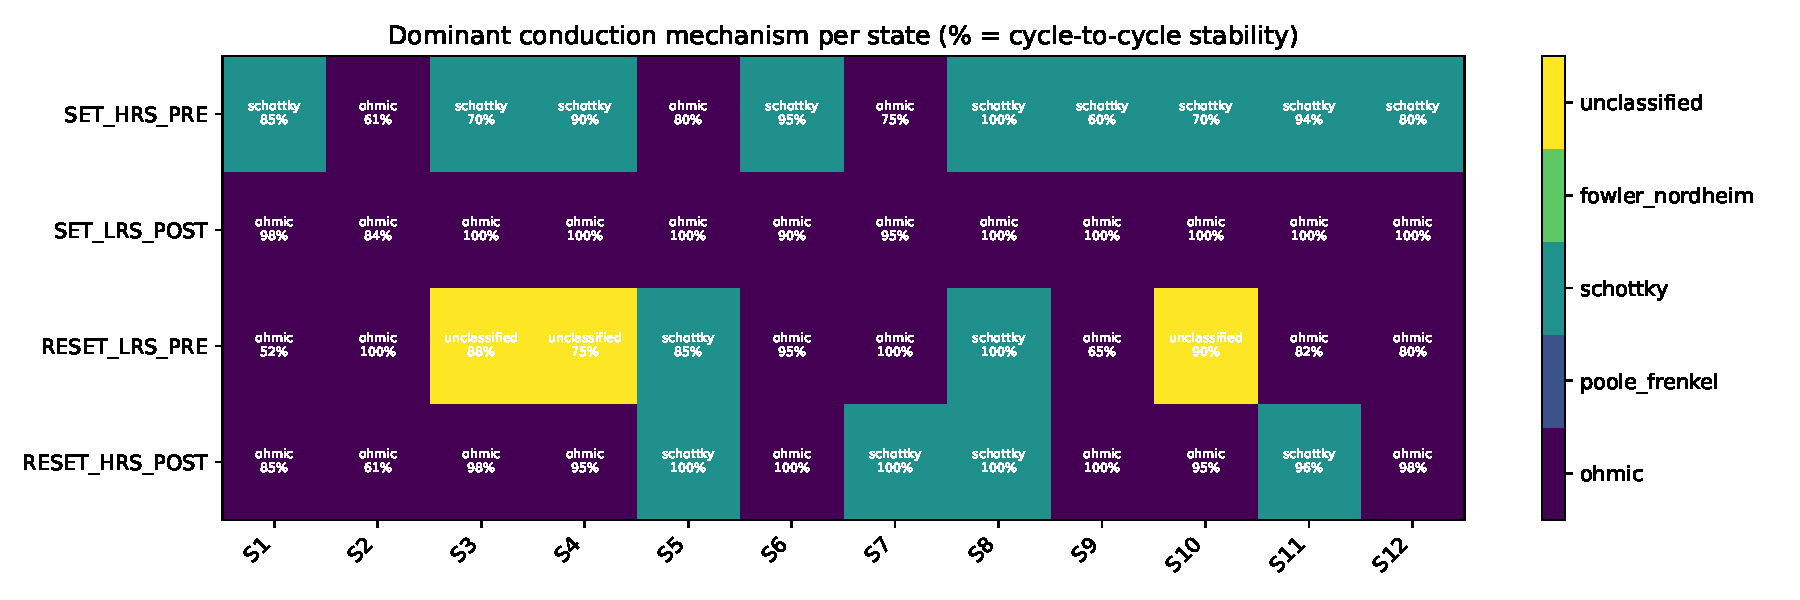
\includegraphics[width=0.98\textwidth]{results/variability/mechanism_map.pdf}
\caption{Dominant conduction mechanism and cycle-to-cycle assignment
stability for each resistance-state segment and deposition condition.  The
post-SET LRS is consistently ohmic, whereas the post-RESET HRS is
Schottky-dominant for all twelve conditions.}
\label{fig:mechanism-map}
\end{figure*}

\subsection{Point-Estimate Fit Quality}
\label{sec:res-fit}

Table~\ref{tab:fitquality} reports the unweighted validation error for every
condition.  The SET branch is reproduced with RMSE from 0.47 to 0.77 decades
(mean 0.530), while RESET is more difficult, with RMSE from 0.65 to 1.02
decades (mean 0.761).  Visually, the model captures the hysteresis order, the
main SET and RESET transitions, the compliance-limited region, and the LRS
return branch.  The largest residuals occur near the SET transition and along
the Schottky-limited HRS approach, where the regime analysis already warned
that the model current law is incomplete.

The Durbin--Watson (DW) statistics are also intentionally reported.  Their
values are well below 2 for all conditions, meaning the residuals are
correlated along the voltage sweep rather than random point-to-point noise.
For a device paper this is useful information: it says the remaining error is
mostly systematic model mismatch, not measurement scatter.  S2 illustrates
the point, with the largest RESET RMSE (1.02 decades), the lowest SET DW, and
the least stable Schottky assignment among the Schottky-dominant pre-SET
conditions.

\begin{table}[!t]
\centering
\caption{Validation fit quality per condition: unweighted RMSE of
$\log_{10}|I|$ (decades) and Durbin--Watson statistics.}
\label{tab:fitquality}
\footnotesize
\begin{tabular}{@{}lcccc@{}}
\toprule
Cond. & RMSE$_{\mathrm{SET}}$ & RMSE$_{\mathrm{RESET}}$ &
DW$_{\mathrm{SET}}$ & DW$_{\mathrm{RESET}}$\\
\midrule
S1  & 0.500 & 0.689 & 0.86 & 0.85\\
S2  & 0.772 & 1.016 & 0.46 & 0.56\\
S3  & 0.566 & 0.659 & 0.72 & 0.98\\
S4  & 0.514 & 0.730 & 0.82 & 0.90\\
S5  & 0.508 & 0.805 & 0.85 & 0.74\\
S6  & 0.468 & 0.650 & 0.94 & 0.93\\
S7  & 0.477 & 0.726 & 1.04 & 0.91\\
S8  & 0.495 & 1.001 & 1.03 & 0.54\\
S9  & 0.510 & 0.700 & 0.92 & 1.04\\
S10 & 0.508 & 0.718 & 1.00 & 0.98\\
S11 & 0.494 & 0.753 & 0.92 & 0.88\\
S12 & 0.548 & 0.681 & 0.96 & 1.01\\
\midrule
Mean & 0.530 & 0.761 & -- & --\\
\bottomrule
\end{tabular}
\end{table}

\subsection{Out-of-Sample Generalization Across Measured Cycles}
\label{sec:res-heldout}

A parameter set fitted to one cycle is useful for circuit simulation only if
it describes the other cycles from the same device.  We test this directly.
The simulated medoid fit is scored point-by-point on the common voltage grid
against every measured cycle, not only against the medoid used during
calibration.  The medoid cycle gives the in-sample RMSE in
Table~\ref{tab:fitquality}; the remaining 19--100 cycles per condition form a
held-out cycle population.

Figure~\ref{fig:heldout} shows the resulting per-cycle RMSE distributions.
Averaged over all conditions, the held-out median RMSE is 0.542 decades for
SET and 0.800 decades for RESET, compared with in-sample means of 0.530 and
0.761 decades.  The average generalization gap is therefore only 0.012
decades for SET and 0.039 decades for RESET.  For every condition, the
in-sample value falls inside the held-out interquartile range.  This is the
key evidence that the fitted compact model represents the measured device
population rather than memorizing one selected trace.

\begin{figure}[!t]
\centering
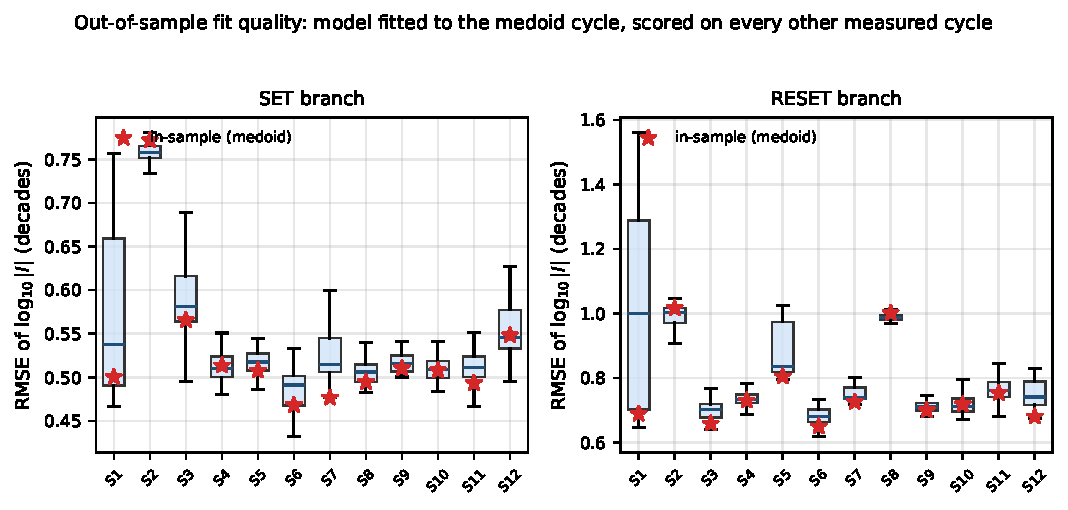
\includegraphics[width=\columnwidth]{results/paper_alt/heldout_rmse.pdf}
\caption{Out-of-sample fit quality.  Box plots: distribution of
$\log_{10}|I|$ RMSE when the model fitted to the medoid cycle is scored
against every other measured cycle of the device (whiskers exclude outliers).
Stars mark the in-sample (medoid) RMSE.  Held-out and in-sample errors are
statistically indistinguishable, evidencing generalization rather than
overfitting.}
\label{fig:heldout}
\end{figure}

Figure~\ref{fig:overlay} shows the same idea for S1 in the time/order of the
sweep.  The fitted curve follows the measured median and stays inside the
cycle-to-cycle envelope for most of the trajectory.  The departures occur at
the SET transition and on the HRS approach.  Across conditions, the fitted SET
curve lies inside the measured min--max band for 77\% of grid points on
average, compared with 63\% for RESET.  The lower RESET coverage is
consistent with the missing Schottky-limited HRS branch identified earlier,
not with overfitting, because RESET is elevated both in-sample and held out.

\begin{figure}[!t]
\centering
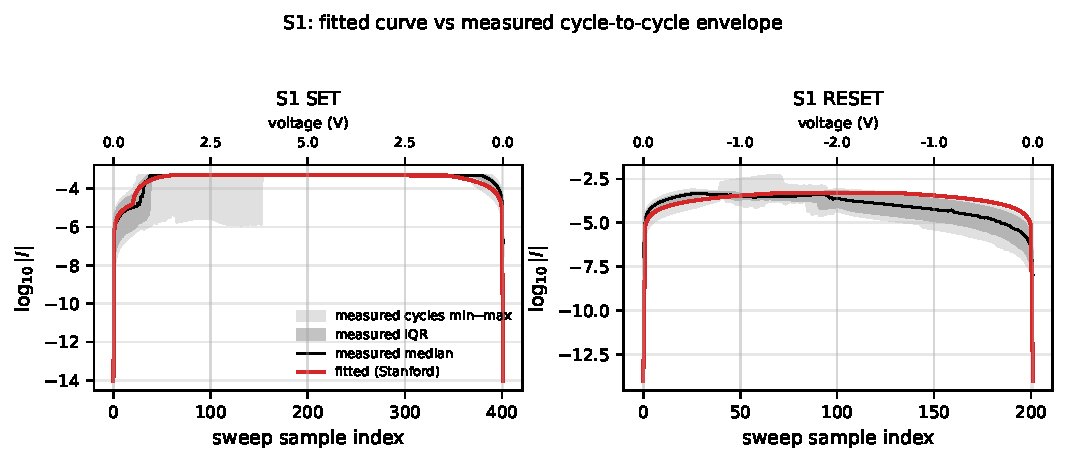
\includegraphics[width=\columnwidth]{results/paper_alt/heldout_overlay_S1.pdf}
\caption{S1 fitted curve (red) against the measured cycle-to-cycle envelope
(min--max and interquartile bands, with the measured median) along the sweep
sequence; the secondary axis marks voltage.  The fit stays within the
measured spread except at the SET transition and the HRS approach.}
\label{fig:overlay}
\end{figure}

\subsection{Identifiability: What DC Data Actually Constrain}
\label{sec:res-ident}

The bootstrap answers a practical extraction question: if the measured cycle
population is sampled again, do we recover the same parameter?  In
Fig.~\ref{fig:param-cv}, each entry is the coefficient of variation (CV) of
the bootstrap distribution for one parameter and one condition.  All 2400
refits (200 draws $\times$ 12 conditions) completed, and all 192
condition--parameter intervals are finite and nondegenerate.  The median CV
over all entries is 0.448, with a range of 0.202--2.698.

The clearest repeatable quantities are the branch voltage scales, with median
CV near 0.28.  This is physically reasonable: the voltage scale controls the
curvature of the measured branch, so the DC butterfly curve directly
constrains it.  By contrast, $R_s$ has a median CV of 1.444, and the SET and
RESET velocity prefactors have median CVs of 1.194 and 1.282.  The current
scale $I_0$ and activation energies also vary substantially.  These
parameters can help the optimizer fit a trace, but the DC data do not recover
them repeatably enough for process interpretation.

The Fisher analysis supports the same broad conclusion but should be read
with caution.  Across conditions, the Fisher condition numbers range from
$6.2\times10^{18}$ to $1.6\times10^{66}$, far beyond what can support precise
per-parameter certification in double precision.  Figure~\ref{fig:ident}
therefore serves as a local sensitivity map rather than the main
identifiability decision.  Where Fisher and bootstrap agree, the conclusion
is strong: branch voltage scales and switching-field combinations are better
determined than $I_0$, $g_0$, activation energies, velocity prefactors, and
gap-geometry parameters.  Where they disagree, the bootstrap is more
important for this device study.  The best example is $R_s$, which can look
locally well determined at one optimum yet varies strongly under cycle
resampling.  A subset of profile-likelihood scans (S1--S4) also returns
``flat/non-identifiable'' behavior for nearly all coordinates, consistent
with the bootstrap reading.

The device-level interpretation is therefore narrow but useful: DC butterfly
data constrain effective branch scales and switching-field combinations more
reliably than they constrain a unique decomposition into current prefactors,
activation energies, gap geometry, and kinetic prefactors.

\begin{figure}[!t]
\centering
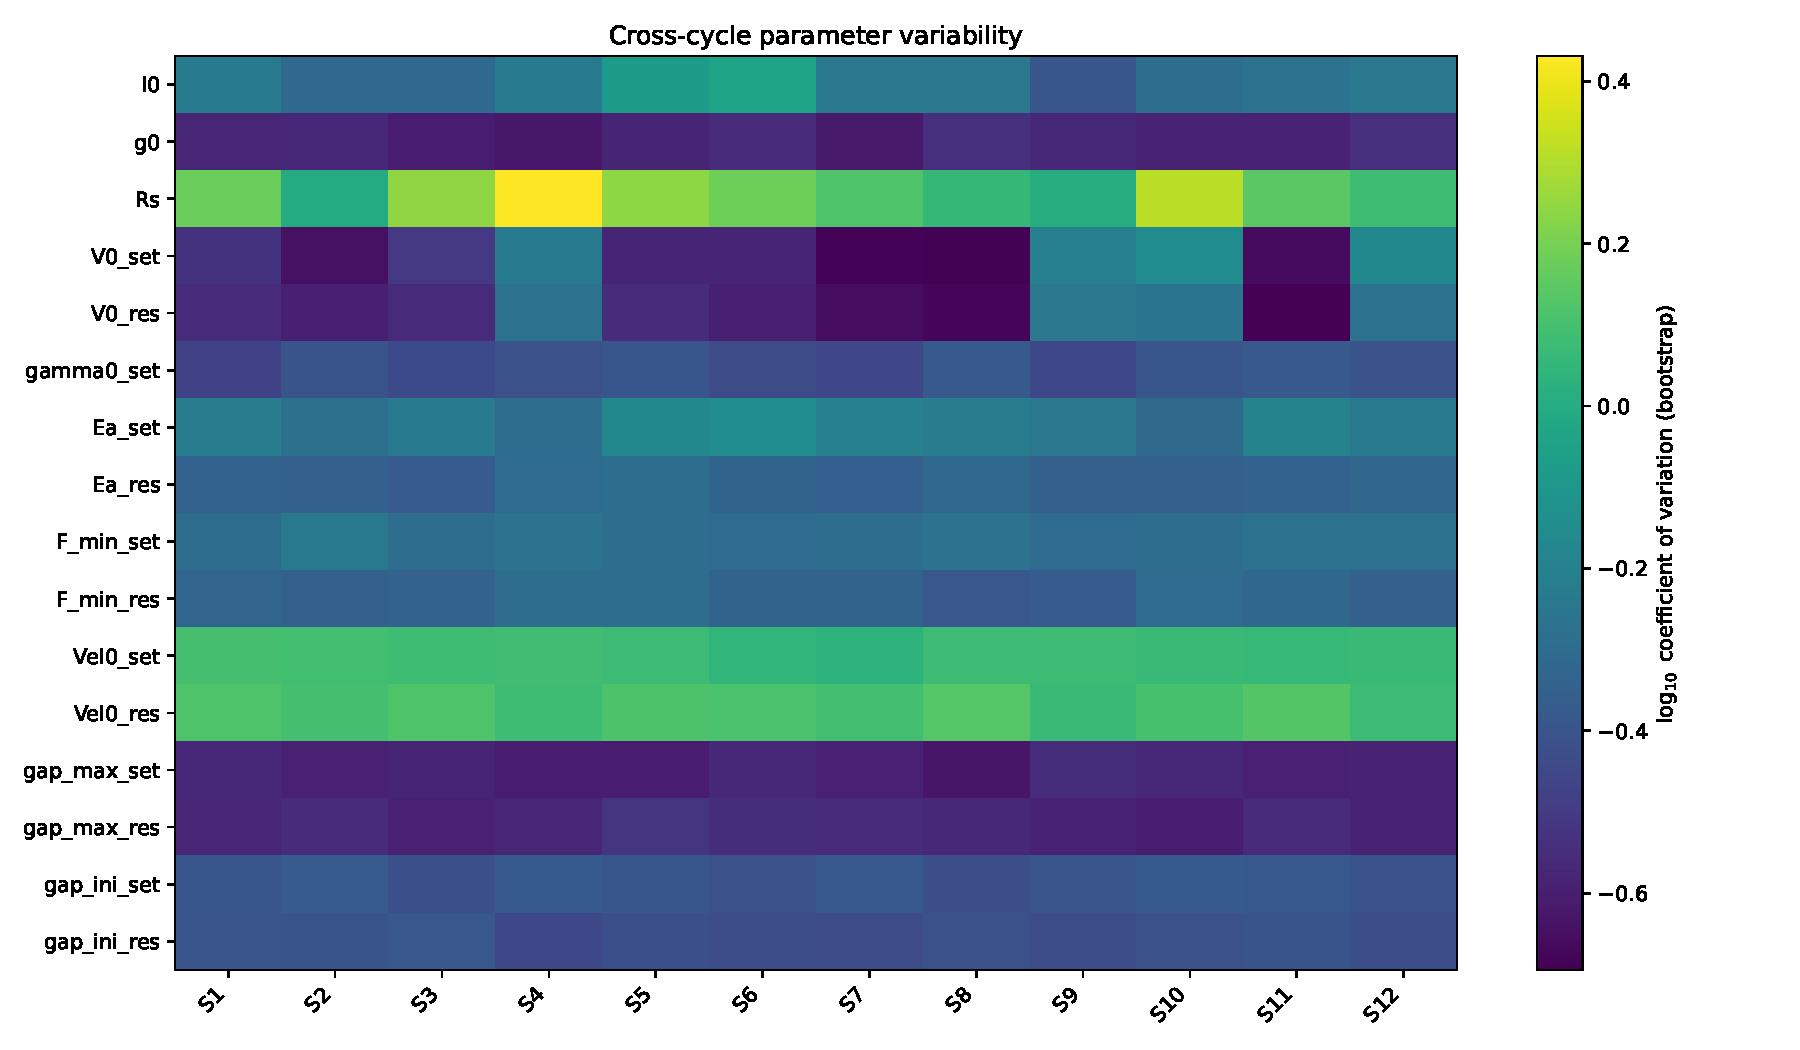
\includegraphics[width=\columnwidth]{results/variability/parameter_cv.pdf}
\caption{Cycle-to-cycle parameter variability from 200 cluster-bootstrap
refits per condition (color: $\log_{10}\mathrm{CV}$).  Branch voltage scales
are comparatively repeatable; series resistance and velocity prefactors are
the least stable.  This bootstrap CV is our primary identifiability evidence.}
\label{fig:param-cv}
\end{figure}

\begin{figure}[!t]
\centering
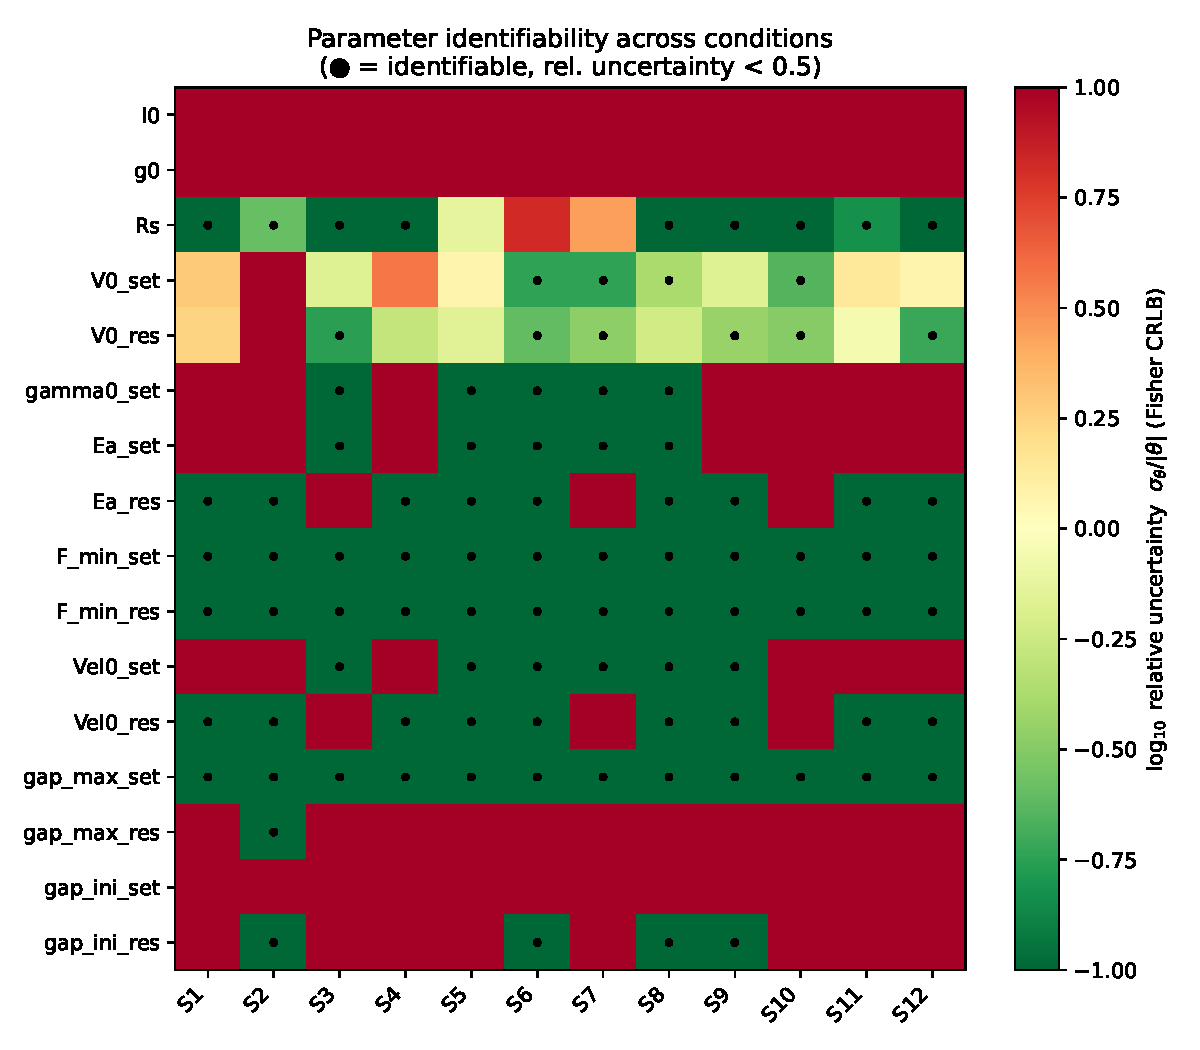
\includegraphics[width=\columnwidth]{results/publication/identifiability_heatmap.pdf}
\caption{Local Fisher relative uncertainty $\sigma_\theta/|\theta|$ (log color
scale) for the 16 active parameters across the twelve conditions, shown as a
corroborating cross-check.  The extremely large condition numbers
($10^{18}$--$10^{66}$) preclude certifying individual coordinates from this
diagnostic alone; conclusions are drawn only where it agrees with
Fig.~\ref{fig:param-cv}.}
\label{fig:ident}
\end{figure}

\subsection{Ablation: What Each Ingredient Buys}
\label{sec:res-ablation}

Table~\ref{tab:ablation} compares the fitting variants using unweighted
validation RMSE.  The most obvious requirement is optimization itself.  On
RESET, using physics-informed prior means without Bayesian optimization gives
$1.528\pm0.434$ decades, while optimized variants are near
$0.756\pm0.124$ decades.  SET is less sensitive because the LRS and
compliance-limited portions are already close to the prior prediction.

The three optimized variants have similar aggregate RMSE.  This is
informative because regime conditioning and informative priors do not mainly
buy a lower overlay error; they keep the fit from using
unsupported Schottky/FN HRS regions to distort parameters that belong to the
Stanford bulk current law.  The ablation therefore reinforces the main
message: a compact-model overlay alone is not enough to establish physical
parameter extraction.  Generalization and identifiability are the quantities
that decide what can be trusted.

\begin{table}[!t]
\centering
\caption{Ablation over all 12 conditions: unweighted validation RMSE
(decades), mean $\pm$ standard deviation across conditions.}
\label{tab:ablation}
\footnotesize
\begin{tabular}{@{}lcc@{}}
\toprule
Variant & RMSE$_{\mathrm{SET}}$ & RMSE$_{\mathrm{RESET}}$\\
\midrule
Regime-conditioned + weighting & $0.530\pm0.081$ & $0.761\pm0.123$\\
Physics priors + BO & $0.546\pm0.077$ & $0.756\pm0.124$\\
Uninformative priors + BO & $0.537\pm0.076$ & $0.755\pm0.126$\\
Physics priors, no BO & $0.571\pm0.115$ & $1.528\pm0.434$\\
\bottomrule
\end{tabular}
\end{table}

\subsection{Deposition-Resolved Extraction}
\label{sec:res-trends}

The deposition DOE in Table~\ref{tab:doe} gives a direct way to use the
identifiability result.  A response surface should only be built from
parameters that are repeatably extracted; otherwise the apparent process
trend may simply be fit ambiguity.  Figure~\ref{fig:trends} compares these
two cases.  The branch voltage scales $V_{0,\mathrm{SET}}$ and
$V_{0,\mathrm{RESET}}$ have relatively tight bootstrap confidence intervals
and vary systematically with deposition.  For example,
$V_{0,\mathrm{RESET}}$ tends to be lower at the 35\% oxygen, low-power
corners (S3 and S4) than at the oxygen-poor corners (S1 and S2).  These
quantities can therefore support deposition-resolved compact-model
interpretation.

Series resistance gives the opposite lesson.  It is often locally sensitive
in the Fisher calculation, but its bootstrap 95\% intervals span one to two
orders of magnitude.  Its apparent changes across conditions cannot be
separated from cycle-to-cycle extraction uncertainty.  For a fabrication or
process study, $R_s$ should therefore not be used as a response-surface
output from these DC sweeps, even if a single fitted curve appears to prefer a
particular value.

\begin{figure}[!t]
\centering
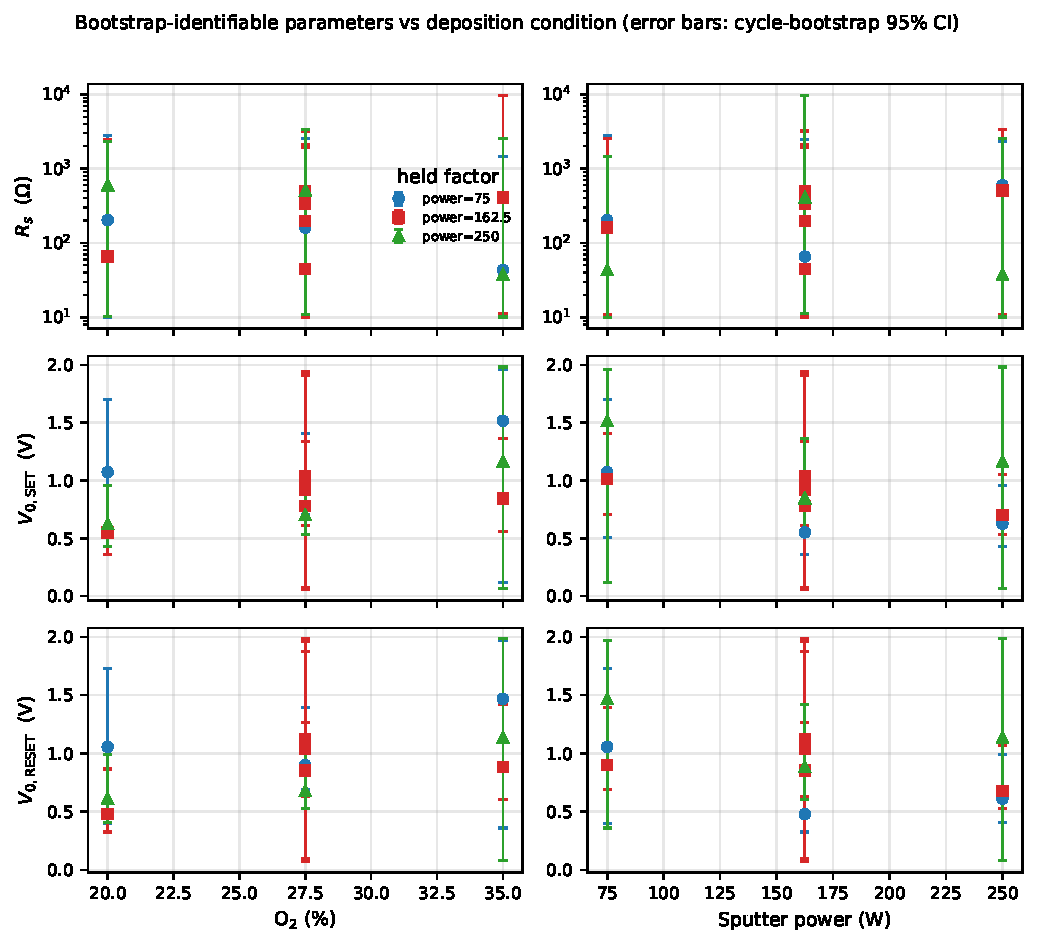
\includegraphics[width=\columnwidth]{results/paper_alt/deposition_trends.pdf}
\caption{Bootstrap-identifiable parameters versus deposition condition (error
bars: cycle-bootstrap 95\% CI).  Branch voltage scales (middle, bottom rows)
are tightly constrained and carry deposition information; series resistance
(top) spans up to two decades and cannot support a response surface despite
being locally Fisher-identifiable.}
\label{fig:trends}
\end{figure}

The regime classifier also provides a process-facing HRS observable that is
not a Stanford-model fitting parameter.  Figure~\ref{fig:schottky} plots the
dynamic relative permittivity inferred from the post-RESET Schottky window.
All twelve conditions fall in the physically admissible range of 4.7--32,
supporting the conclusion that the post-RESET HRS is interface-limited across
the entire DOE.  The approximately three-fold scatter among the replicated
center-point devices (S9--S12) further suggests that the interface response
has its own device-to-device and cycle-to-cycle variability, not just a
single-valued dependence on the nominal deposition setpoint.  This is an
automated, quantitative extension of mechanism analysis that was previously
performed manually \cite{chowdhury2025mwscas}.

\begin{figure}[!t]
\centering
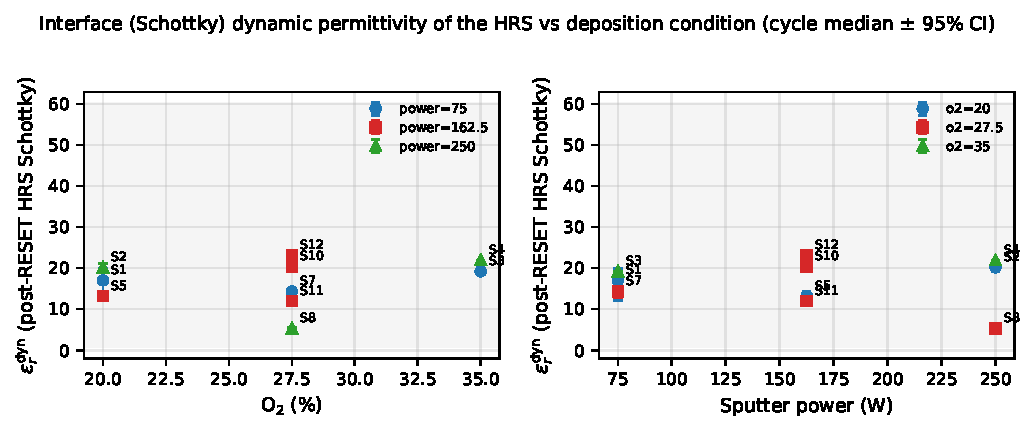
\includegraphics[width=\columnwidth]{results/paper_alt/hrs_schottky_trend.pdf}
\caption{Dynamic relative permittivity inferred from the post-RESET HRS
Schottky window for all twelve conditions, versus oxygen (left) and power
(right).  Shaded band: admissibility interval $[1,60]$.  All conditions are
physically admissible, corroborating interface-limited HRS conduction
device-wide.}
\label{fig:schottky}
\end{figure}

% =========================================================================
\section{Discussion}
\label{sec:discussion}
% =========================================================================

\subsection{Implications for Compact-Model Users}

For circuit users, the result is encouraging but bounded.  The calibrated
Stanford parameter files are useful behavioral descriptions for the measured
DC protocol: a fit obtained from one representative cycle predicts the other
cycles of the same device with essentially the same error.  This supports
their use in circuit-level studies that need a compact description of the
observed switching loops.

For device and fabrication interpretation, the message is more selective.
Only repeatable parameter combinations should be compared across deposition
conditions.  In this data set, the branch voltage scales and related
switching-field combinations pass that test.  Fitted $E_a$, $\nu_0$, gap
geometry, and even $R_s$ do not have enough cycle-bootstrap repeatability to
be treated as standalone physical outputs from DC sweeps.  Reporting the full
parameter table is still useful for reproducibility, but the process
discussion should be based on the identifiable subset.

\subsection{Model Adequacy for TaO$_x$}

The regime analysis also explains why RESET remains harder to fit than SET.
The post-RESET HRS is Schottky-dominant in nearly all cycles, while the
released Stanford model uses a single bulk-like $\sinh$ current law.  The
remaining RESET error is therefore a model-adequacy issue, not simply an
optimizer issue.  This interpretation is supported by the ablation study,
where the optimized variants reach similar unweighted RMSE, and by the
held-out test, where RESET error is elevated both in-sample and out of
sample.

A natural next model extension would add a barrier-limited HRS branch or a
gap-dependent barrier term \cite{chiu2014,bocquet2014,bengel2020jart}.  The
regime map gives the experimental windows and slopes that such an extension
should target.  Until then, the present flow keeps the Schottky mismatch
visible in the unweighted validation metrics while preventing those regions
from dominating extraction of parameters associated with the Stanford bulk
law.

\subsection{Limitations}

Several limitations should be kept explicit.  First, the transient replay is
quasi-static, so kinetic parameters absorb the effective measurement time
scale; pulsed or sweep-rate-resolved data would be needed to constrain
kinetics more directly \cite{ielmini2016}.  Second, the bootstrap and
out-of-sample analyses are cycle-level analyses for one selected device per
condition.  They quantify cycle-to-cycle variability under the fitting
protocol, not full device-to-device or wafer-level variability, although the
replicated center points give an initial view of that spread.  Third, Fisher
analysis is used only as a local cross-check, and profile-likelihood scans
were completed for a subset of conditions (S1--S4); a future release should
complete those scans for all conditions using a common optimum.  Finally, the
reset-side $\gamma_0$ is structurally overridden under negative bias in the
released Verilog-A model, so it is retained for compatibility but not
physically interpreted.

% =========================================================================
\section{Conclusion}
\label{sec:conclusion}
% =========================================================================

We presented a device-guided extraction flow for the Stanford RRAM compact
model and applied it to twelve sputter-deposited TaO$_x$ deposition
conditions.  The fitted models reproduce the measured DC switching loops with
mean RMSE of 0.530 decades for SET and 0.761 decades for RESET.  More
importantly, the fits generalize across measured cycles: when a model fitted
to one representative cycle is scored against all other cycles from the same
device, the held-out median RMSE remains close to the in-sample value
(0.542/0.800 decades for SET/RESET).

The extracted parameter table should not be interpreted uniformly.  Cycle
bootstrap shows that branch voltage scales are repeatable and carry usable
deposition trends, while series resistance, velocity prefactors, activation
energies, and several gap-related parameters are not repeatable enough for
standalone physical interpretation from these DC sweeps.  The regime analysis
adds the corresponding device-physics reason for the residual floor: the
post-RESET HRS is Schottky-dominant in 92.5--100\% of cycles, with admissible
dynamic permittivities, while the released Stanford current law does not
explicitly include that interface-limited branch.  For RRAM compact-model
calibration, fit quality should therefore be reported together with
cycle-level generalization, parameter identifiability, and conduction-regime
validity.

% =========================================================================
\begin{thebibliography}{99}\footnotesize

\bibitem{wong2012metal}
H.-S.~P. Wong \emph{et~al.}, ``Metal-oxide RRAM,'' \emph{Proc. IEEE},
vol.~100, no.~6, pp. 1951--1970, Jun. 2012.

\bibitem{ielmini2018inmemory}
D.~Ielmini and H.-S.~P. Wong, ``In-memory computing with resistive switching
devices,'' \emph{Nature Electron.}, vol.~1, pp. 333--343, 2018.

\bibitem{yu2018neuro}
S.~Yu, ``Neuro-inspired computing with emerging nonvolatile memories,''
\emph{Proc. IEEE}, vol.~106, no.~2, pp. 260--285, Feb. 2018.

\bibitem{guan2012spice}
X.~Guan, S.~Yu, and H.-S.~P. Wong, ``A SPICE compact model of metal oxide
resistive switching memory with variations,'' \emph{IEEE Electron Device
Lett.}, vol.~33, no.~10, pp. 1405--1407, Oct. 2012.

\bibitem{jiang2016verification}
Z.~Jiang \emph{et~al.}, ``A compact model for metal--oxide resistive random
access memory with experiment verification,'' \emph{IEEE Trans. Electron
Devices}, vol.~63, no.~5, pp. 1884--1892, May 2016.

\bibitem{bocquet2014}
M.~Bocquet \emph{et~al.}, ``Robust compact model for bipolar oxide-based
resistive switching memories,'' \emph{IEEE Trans. Electron Devices}, vol.~61,
no.~3, pp. 674--681, Mar. 2014.

\bibitem{bengel2020jart}
C.~Bengel \emph{et~al.}, ``Variability-aware modeling of filamentary
oxide-based bipolar resistive switching cells using SPICE level compact
models,'' \emph{IEEE Trans. Circuits Syst. I, Reg. Papers}, vol.~67, no.~12,
pp. 4618--4630, Dec. 2020.

\bibitem{kvatinsky2015vteam}
S.~Kvatinsky \emph{et~al.}, ``VTEAM: A general model for voltage-controlled
memristors,'' \emph{IEEE Trans. Circuits Syst. II, Exp. Briefs}, vol.~62,
no.~8, pp. 786--790, Aug. 2015.

\bibitem{transtrum2015sloppiness}
M.~K. Transtrum \emph{et~al.}, ``Perspective: Sloppiness and emergent theories
in physics, biology, and beyond,'' \emph{J. Chem. Phys.}, vol. 143, no.~1,
Art. no. 010901, 2015.

\bibitem{gutenkunst2007}
R.~N. Gutenkunst \emph{et~al.}, ``Universally sloppy parameter sensitivities in
systems biology models,'' \emph{PLoS Comput. Biol.}, vol.~3, no.~10,
pp. 1871--1878, 2007.

\bibitem{raue2009}
A.~Raue \emph{et~al.}, ``Structural and practical identifiability analysis of
partially observed dynamical models by exploiting the profile likelihood,''
\emph{Bioinformatics}, vol.~25, no.~15, pp. 1923--1929, 2009.

\bibitem{chis2011}
O.-T. Chis, J.~R. Banga, and E.~Balsa-Canto, ``Structural identifiability of
systems biology models: A critical comparison of methods,'' \emph{PLoS ONE},
vol.~6, no.~11, Art. no. e27755, 2011.

\bibitem{chiu2014}
F.-C. Chiu, ``A review on conduction mechanisms in dielectric films,''
\emph{Adv. Mater. Sci. Eng.}, vol. 2014, Art. no. 578168, 2014.

\bibitem{ielmini2016}
D.~Ielmini, ``Resistive switching memories based on metal oxides: Mechanisms,
reliability and scaling,'' \emph{Semicond. Sci. Technol.}, vol.~31, no.~6,
Art. no. 063002, 2016.

\bibitem{wouters2015}
D.~J. Wouters, R.~Waser, and M.~Wuttig, ``Phase-change and redox-based
resistive switching memories,'' \emph{Proc. IEEE}, vol.~103, no.~8,
pp. 1274--1288, Aug. 2015.

\bibitem{snoek2012practical}
J.~Snoek, H.~Larochelle, and R.~P. Adams, ``Practical Bayesian optimization
of machine learning algorithms,'' in \emph{Proc. Adv. Neural Inf. Process.
Syst. (NeurIPS)}, 2012, pp. 2951--2959.

\bibitem{shahriari2016}
B.~Shahriari \emph{et~al.}, ``Taking the human out of the loop: A review of
Bayesian optimization,'' \emph{Proc. IEEE}, vol.~104, no.~1, pp. 148--175,
Jan. 2016.

\bibitem{efron1994bootstrap}
B.~Efron and R.~J. Tibshirani, \emph{An Introduction to the Bootstrap}.
New York, NY, USA: Chapman \& Hall/CRC, 1994.

\bibitem{chowdhury2025mwscas}
M.~T.~R. Chowdhury, A.~Moazzeni, and G.~Tutuncuoglu, ``Atomic-scale insights
into the switching mechanisms of RRAM devices,'' in \emph{Proc. IEEE 68th
Int. Midwest Symp. Circuits Syst. (MWSCAS)}, Lansing, MI, USA, 2025,
pp. 518--522.

\bibitem{moazzeni2023}
A.~Moazzeni, M.~T.~R. Chowdhury, and G.~Tutuncuoglu, ``The impact of
operation conditions on potentiation, depression and endurance dynamics of
tantalum oxide RRAMs,'' in \emph{Proc. IEEE Int. Integr. Rel. Workshop
(IIRW)}, 2023.

\bibitem{lee2011fast}
M.-J. Lee \emph{et~al.}, ``A fast, high-endurance and scalable non-volatile
memory device made from asymmetric Ta$_2$O$_{5-x}$/TaO$_{2-x}$ bilayer
structures,'' \emph{Nature Mater.}, vol.~10, pp. 625--630, 2011.

\end{thebibliography}

\end{document}
